\subsection{Free Energy}
\begin{frame}{Free energy calculation}
To use the \enquote{MMPBSA.py} code, you first need to split the parameter file into:
\begin{itemize}
	\item Complex (no solvent)
	\item Receptor (ligand, Mg\textsuperscript{2+} and diphosphate ions)
	\item Ligand
\end{itemize}
\vspace{3cm}
This can be done using \enquote{ante-MMPBSA.py}

{\tiny Further reading: \href{https://ambermd.org/tutorials/advanced/tutorial3/}{https://ambermd.org/tutorials/advanced/tutorial3/}}
\end{frame}

\begin{frame}{Free energy calculation}
\begin{figure}
\centering
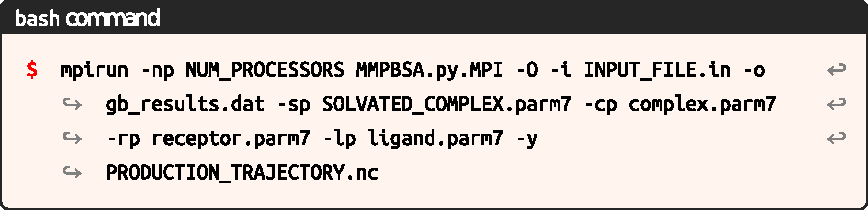
\includegraphics[width=0.8\textwidth]{figures/dynamics/gbsa.pdf}
\end{figure}
\end{frame}